\documentclass[12pt]{beamer}

\usepackage[utf8]{inputenc}
\usepackage[brazilian]{babel} % Defini o idioma utilizado
\usepackage{xcolor}  % Permite o uso de cores no texto

\definecolor{LightCyan}{rgb}{0.88,1,1} %Cria uma nova cor usando o código RGB
\definecolor{DarkBlue}{RGB}{41, 4, 135} %Cria uma nova cor usando o código RGB

\renewcommand{\baselinestretch}{1.2}
\setlength\parindent{5.5mm}

\renewcommand{\b}[1]{\textbf{#1}}
\newcommand{\blue}[1]{\textcolor{blue}{#1}}
\newcommand{\blueb}[1]{\textbf{\textcolor{blue}{#1}}}

\newcommand{\inn}{$\in \mathbb{N}$ \ } % Abreviação para "no conjunto dos naturais".
\newcommand{\inz}{$\in \mathbb{Z}$ \ } % Abreviação para "no conjunto dos inteiros".

\newcommand{\imp}{$\Rightarrow$ \ } 

% Link para o site: https://hartwork.org/beamer-theme-matrix/
\usetheme{Berlin} % Nome do tema
\usecolortheme{orchid} % Esquema de cores

%Personalizar o modelo
\setbeamercolor{title}{fg = LightCyan, bg= DarkBlue } % Muda a letra e o fundo do título

% \setbeamercolor{block title alerted}{fg=white ,bg= pink}
% \setbeamercolor{block body alerted}{bg= pink !10}
% \setbeamercolor{block title}{fg=black ,bg= yellow}
% \setbeamercolor{block body}{bg= yellow !20}

%Informações da capa
\title{Análise de dados}
\author[Gabriel H.]{Gabriel Henrique do Nascimento Neres}
\institute[CEUB]{CEUB}
\date{\today}


\begin{document}
\maketitle

% \begin{frame}{Sumário}  % Cria um sumário da apresentação
% \tableofcontents
% \end{frame}

\section{Obtenção dos dados}
\begin{frame}{Aquisição}
  Os dados utilizados foram sobre Energia armazenada (EAR) e Consumo de energia elétrica no Brasil, obtidos em https://basedosdados.org/, acessados utilizando o Google BigQuery.
  \begin{columns}[t]
    \begin{column}{6cm}
      \begin{figure}[h]
        \begin{center}
          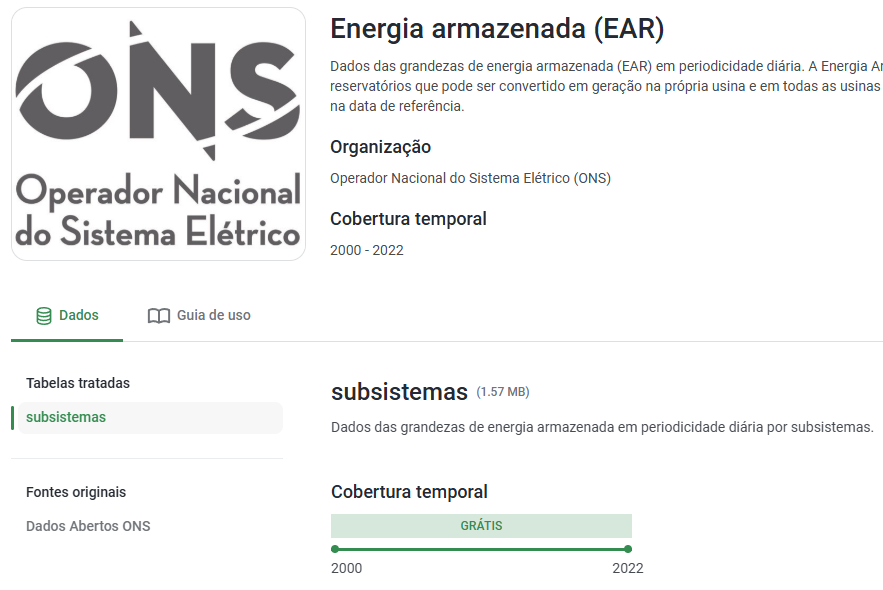
\includegraphics[width=\linewidth]{EAR.png}
        \end{center}
      \end{figure}
    \end{column}
    \begin{column}{6cm}
      \begin{figure}[h]
        \begin{center}
          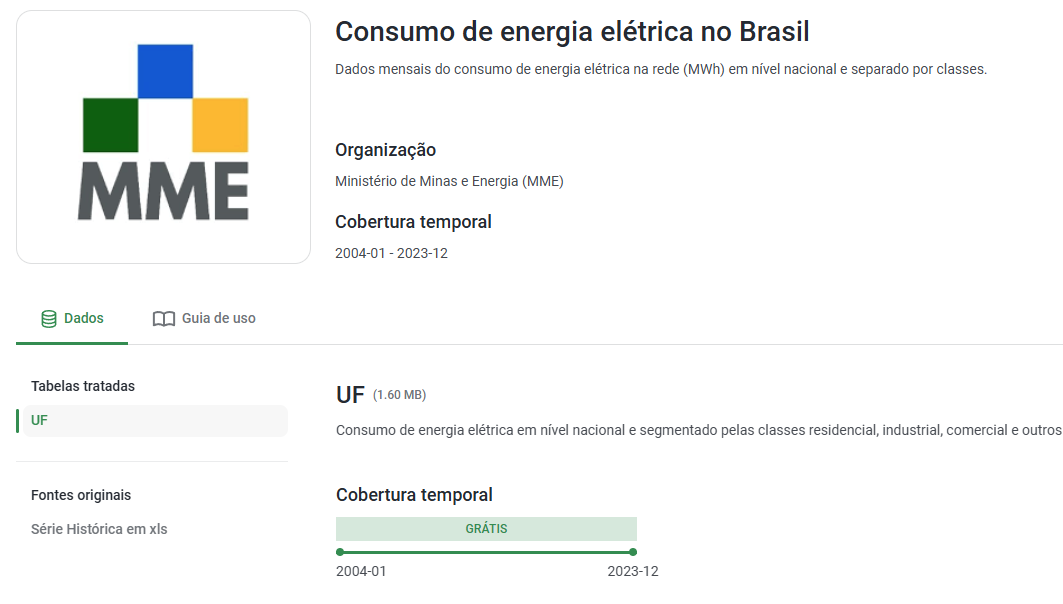
\includegraphics[width=\linewidth]{Consumo Energia.png}
        \end{center}
      \end{figure}
    \end{column}
  \end{columns}
\end{frame}

\begin{frame}{Preparação — Integração}
  Para integrar às duas fontes de dados foi preciso:
  \begin{itemize}
    \item Restringir o intervalo de tempo;
    \begin{itemize}
      \item Ano entre 2010 e 2022.
    \end{itemize}
    \item Os dados da EAR precisaram ser unificados por mês (media do mês);
    \begin{itemize}
      \item Quebra a coluna data em mês e ano e calcula a média das outras colunas.
    \end{itemize}
    \item Os dados do consumo elétrico precisaram ser unificados por região;
  \end{itemize}
\end{frame}

\begin{frame}{Preparação — Limpeza}
  Dentre as colunas escolhidas, foi preciso reescalonar as unidades de medida de energia entre os dois bancos, pois um estava em MWh por mês e o outro MWmês. Para isso, foi preciso  dividir o valor de MWh por mês por 720 para converter para MWmês.
\end{frame}

\section{Análise dos dados}
\begin{frame}{Análise dos dados}
A categoria de dado em cada uma das colunas escolhidas são:
  \begin{itemize}
    \item Ano: Numérico discreto.
    \item Mes: Numérico discreto.
    \item Maxima Energia Armazenada: Numérico contínuo.
    \item Energia Armazenada Verificada: Numérico contínuo.
    \item Porcentagem Armazenamento Total: Numérico contínuo.
    \item Subsistema: Categórica nominal.
    \item Consumo Mensal: Numérico contínuo.
  \end{itemize}  
\end{frame} 

\begin{frame}{Análise dos dados}
  O campo escolhido para análise foi a Consumo Mensal.
  \begin{itemize}
    \item Média: 1.103.791,4
    \item Desvio Padrão: 854.403,7
    \item Coeficiente de Variação: 77,4
    \item Mediana: 790.793,64
    \item Moda: Apenas valores únicos, mesmo com Floor.
    \item Quartis:
    \begin{itemize}
      \item 25\%: 481.443,95
      \item 50\%: 790.793,64
      \item 75\%: 1.533.716,23
    \end{itemize}
  \end{itemize}
\end{frame}

\begin{frame}{Outliers}
  Ao analisar o Z-score da coluna Consumo Mensal, não foi encontrado nenhum outlier seguindo como parâmetro algum valor acima de 3 ou menor que -3. O intervalo encontrado foi entre 2 e -1. Para garantir que não houvesse algum outlier nas demais colunas foi feito o mesmo procedimento para elas.  
\end{frame}

\begin{frame}{Outliers}
\begin{columns}[t]
  \begin{column}{6,5cm}
    \begin{itemize}
      \item Energia Armazenada Verificada:
      \begin{itemize}
        \item Nordeste: 2,2 e -1,7;
        \item Sul: 1,7 a -2,2;
        \item Sudeste / Centro-Oeste: 2,4 e -1.5;
        \item Norte: 1,6 e -1,9.
      \end{itemize}
    \end{itemize}  
    \end{column}
  \begin{column}{6,5cm}
    \begin{itemize}
      \item Maxima Energia Armazenada:
      \begin{itemize}
        \item Nordeste: 0,9 e -1,4;
        \item Sul: 0,8 e -2,7;
        \item Sudeste / Centro-Oeste: 0,8 e -3,8;
        \item Norte: 0,6 e -1,8.
      \end{itemize}
    \end{itemize}  
  \end{column}
\end{columns}
\end{frame}

\section{Gráficos}
\begin{frame}{Gráficos}
  Para ver a evolução do consumo temporalmente, podemos utilizar o gráfico de dispersão ou o de linhas.

\begin{figure}[h]
  \begin{center}
    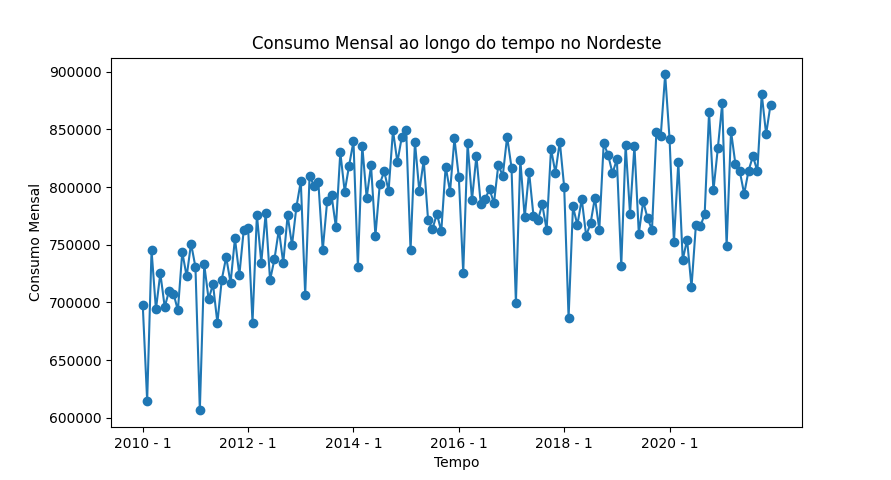
\includegraphics[width=0.85\linewidth]{Consumo_mensal.png}
  \end{center}
\end{figure}
\end{frame}

\begin{frame}
  Análise do gasto total do período de 2010 a 2022 de cada região.

\begin{figure}[h]
  \begin{center}
    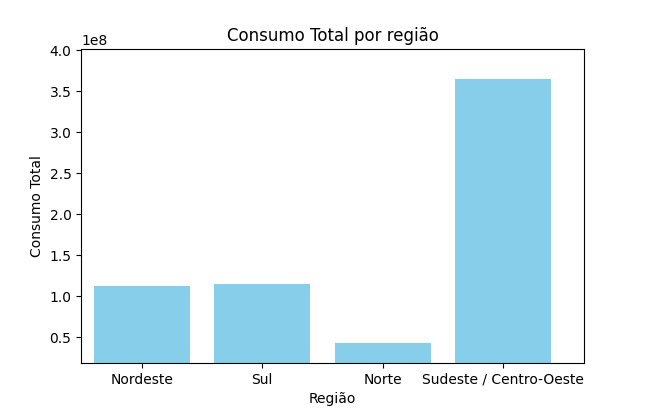
\includegraphics[width=0.9\linewidth]{Consumo_Total.png}
  \end{center}
\end{figure}
\end{frame}

\begin{frame}
\begin{columns}
  \begin{column}{5cm}
    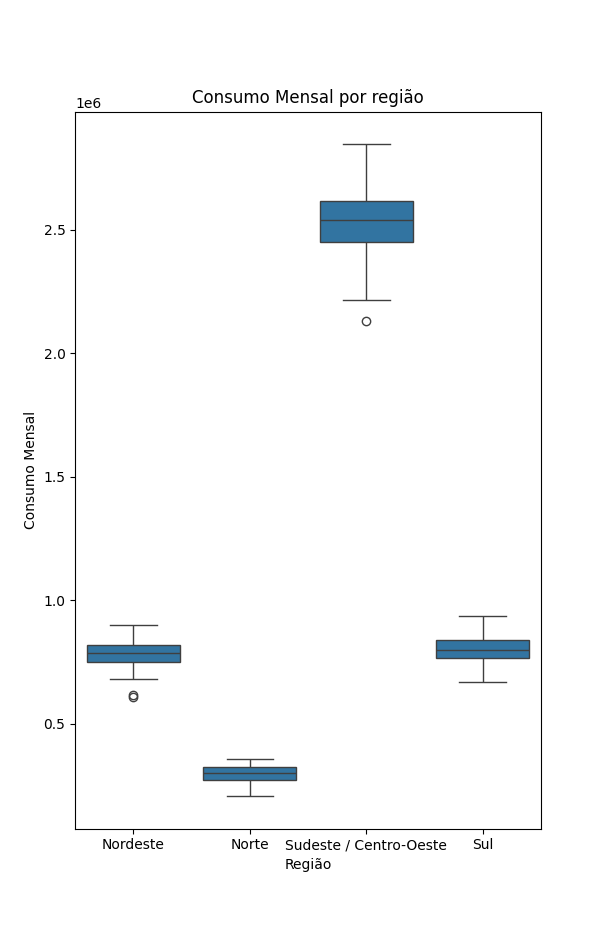
\includegraphics[width=\linewidth]{Consumo_mensal_boxPlot.png}
  \end{column}
  \begin{column}{6cm}
    Análise do gasto mensal de cada região utilizando o Box Plot.
  \end{column}
\end{columns}
\end{frame}

\section{Referências bibliográficas}
\begin{frame}{Referências bibliográficas}
  https://basedosdados.org/dataset/0a54258d-4adc-4fa9-a7c8-8e39426d22a2?table=d4185bb5-7aeb-41f1-9bcd-e081f7eb8abc
  https://basedosdados.org/dataset/3e31e540-81ba-4665-9e72-3f81c176adad?table=b955feef-1649-428b-ba46-bc891d2facc2
  https://www.ons.org.br/sites/multimidia/Documentos\%20Compartilhados/dados/DADOS2014\_ONS/9\_1.html
\end{frame}


% \section{Comandos}
% \subsection{Pause}
% \begin{frame} % Para inciar um frame
% \frametitle{Uso do pause} %Determina o título do frame
% Existe um comando em \LaTeX chamado \textcolor{blue}{pause} que pode parar uma apresentação.\pause \ Com ele o restante de um texto só aparece após passar o slide.
% \end{frame}

% \subsection{Colunas}
% \begin{frame}
% \frametitle{Uso de colunas} 
% \begin{columns}
% \column{0.2\textwidth} % largura da primeira coluna
% \begin{itemize}
%    \item Item 1
%    \item Item 2
%    \item Item 3
% \end{itemize}
% \column{0.3\textwidth} % largura da segunda coluna
% Esta é a segunda coluna
% \column{0.4\textwidth} % largura da terceira coluna
% Esta é a terceira coluna
% \end{columns}

% \end{frame}

% \section{Blocos}
% \subsection{Normal}
% \begin{frame}{Bloco Normal}
%    Pode ser usados para \alert{realsar} partes do texto.
%    \begin{block}{Título do Bloco}
%       Isso é um bloco de texto
%    \end{block}
% \end{frame}

% \subsection{Alerta}
% \begin{frame}{Bloco de Alerta}
%    \begin{alertblock}{Título do Bloco de
% alerta}
%       Isso é um bloco de alerta .
%    \end{alertblock}
% \end{frame}

% \subsection{Exemplo}
% \begin{frame}{Bloco de Exemplo}
%    \begin{examples}
%       Isso é um bloco de exemplo .
%    \end{examples}
% \end{frame}



\end{document}